\documentclass{article}
\usepackage[utf8]{inputenc}
\usepackage[english, spanish]{babel}
\usepackage[dvips]{graphics}
\usepackage{amsmath}
\usepackage{amssymb}
\usepackage{fullpage}
\usepackage{epsfig}
\usepackage{multicol}
\usepackage{wasysym}

\usepackage[usenames,dvipsnames]{xcolor} 
\usepackage{hyperref} 
\definecolor{linkcolour}{rgb}{0,0.2,0.6} 
\hypersetup{colorlinks,breaklinks,urlcolor=linkcolour,linkcolor=linkcolour} 

\parindent 0pt
\parskip 0pt

\newcommand{\bbZ}{\mathbb{Z}}


\begin{document}


\includegraphics[width=2cm]{uc.png}
\vspace*{-1.9cm}

\hspace*{2.1cm}
 \begin{tabular}{l}
  \sc Pontificia Universidad Católica de Chile \\
  \sc Escuela de Ingeniería \\
  \sc Departamento de Ciencia de la Computación
  %\vspace{15\baselineskip}\mbox{}
  %\vspace{-3mm}\mbox{}
 \end{tabular}
 \bigskip

\vspace*{5mm}
\begin{center}
{IIC2413 --- Bases de Datos --- 2' 2019} \\
\vspace{3mm}
{\Large\bf Entrega 2} \\
\vspace{2mm}
Matías Reyes \\
Nicolás Van Sint Jan
\end{center}

\section{Diagrama E/R}

\begin{figure}[h]	
	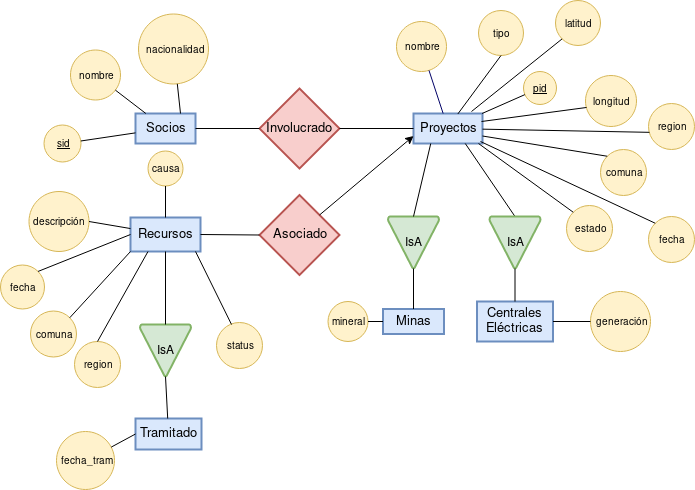
\includegraphics[scale=0.60]{ER_v1.png}
	\caption{Diagrama Entidad/Relación}
\end{figure}

\section{Esquema}

	\begin{itemize}
		\item \texttt{Socios(\underline{nombre}: string, \underline{apellido}: string, nacionalidad: string)} 
		\item \texttt{Proyectos(\underline{nombre}: string, latitud: float, longitud: float, comuna: string,\\ fecha\_apertura: string, operativo: string)} 
		\item \texttt{Recursos(\underline{numero}: string, causa: string, area\_influencia: float, descripcion: string,\\ fecha\_apertura: string, comuna\_tramitacion: string, status: string)}
		\item \texttt{RyP(\underline{numero\_recurso}: string, nombre\_proyecto: string)} 
		
		\item \texttt{SyP(nombre\_socio: string, apellido\_socio: string, nombre\_proyecto: string)} 
		 
		\item \texttt{Mineras(\underline{nombre\_proyecto}: string, mineral: string)} 
		\item \texttt{Centrales(\underline{nombre\_proyecto}: str, tipo generacion: string)} 
		\item \texttt{Tramitados(\underline{numero\_recurso}: string, fecha\_dictamen: string)} 
		
		\item \texttt{CyR(\underline{comuna}: string, region: string)} 
	\end{itemize}

\textbf{BCNF:} %explicacion de porque esta en BCNF

\section{Comandos usados para crear tablas}

\begin{verbatim}
DROP TABLE IF EXISTS Socios;
CREATE TABLE Socios(
	snombre VARCHAR(100),
	apellido VARCHAR(100),
	nacionalidad VARCHAR(100));
\COPY Socios FROM 'psql_socios.csv' DELIMITERS ',' CSV HEADER;


DROP TABLE IF EXISTS Proyectos;
CREATE TABLE Proyectos(
	tipo VARCHAR(20),
	pnombre VARCHAR(100) PRIMARY KEY, 
	latitud FLOAT, 
	longitud FLOAT, 
	comuna VARCHAR(50), 
	fecha_apertura DATE, 
	operativo BOOLEAN);
\COPY Proyectos FROM 'psql_proyectos.csv' DELIMITERS ',' CSV HEADER;


DROP TABLE IF EXISTS Recursos;
CREATE TABLE Recursos(
	numero CHAR(14) PRIMARY KEY, 
	causa VARCHAR(100), 
	area FLOAT, 
	descripcion TEXT, 
	fecha_apertura DATE, 
	comuna VARCHAR(50), 
	status VARCHAR(20));
\COPY Recursos FROM 'psql_recursos.csv' DELIMITERS ',' CSV HEADER;

DROP TABLE IF EXISTS Mineras;
CREATE TABLE Mineras(
	mineral VARCHAR(50), 
	pnombre VARCHAR(100) PRIMARY KEY, 
	FOREIGN KEY (pnombre) REFERENCES Proyectos (pnombre) ON DELETE CASCADE);
\COPY Mineras FROM 'psql_mineras.csv' DELIMITERS ',' CSV HEADER;

DROP TABLE IF EXISTS Comunas;
CREATE TABLE Comunas(
	comuna VARCHAR(50) PRIMARY KEY, 
	region VARCHAR(100));
\COPY Comunas FROM 'psql_comunas.csv' DELIMITERS ',' CSV HEADER;

DROP TABLE IF EXISTS Centrales;
CREATE TABLE Centrales(
	pnombre VARCHAR(100) PRIMARY KEY, 
	generacion VARCHAR(50),  
	FOREIGN KEY (pnombre) REFERENCES Proyectos (pnombre) ON DELETE CASCADE);
\COPY Centrales FROM 'psql_centrales.csv' DELIMITERS ',' CSV HEADER;

DROP TABLE IF EXISTS Tramitados;
CREATE TABLE Tramitados(
	fecha_dictamen DATE, 
	numero CHAR(14) PRIMARY KEY, 
	FOREIGN KEY (numero) REFERENCES Recursos (numero) ON DELETE CASCADE);
\COPY Tramitados FROM 'psql_tramitados.csv' DELIMITERS ',' CSV HEADER;

DROP TABLE IF EXISTS SociosProyectos;
CREATE TABLE SociosProyectos(
	apellido VARCHAR(100), 
	pnombre VARCHAR(100), 
	snombre VARCHAR(100), 
	FOREIGN KEY (apellido, snombre) REFERENCES Socios (apellido, snombre) ON DELETE CASCADE,
	FOREIGN KEY (pnombre) REFERENCES Proyectos (pnombre) ON DELETE CASCADE);
\COPY SociosProyectos FROM 'psql_syp.csv' DELIMITERS ',' CSV HEADER;

DROP TABLE IF EXISTS RecursosProyectos;
CREATE TABLE RecursosProyectos(
	numero CHAR(14) PRIMARY KEY,
	pnombre VARCHAR(100), 
	FOREIGN KEY (pnombre) REFERENCES Proyectos (pnombre) ON DELETE CASCADE,
	FOREIGN KEY (numero) REFERENCES Recursos (numero) ON DELETE CASCADE);
\COPY RecursosProyectos FROM 'psql_ryp.csv' DELIMITERS ',' CSV HEADER;
\end{verbatim}


\section{Consultas}

\begin{enumerate}
	\item \begin{verbatim}
SELECT pnombre FROM Centrales
WHERE generacion='termoeléctrica';
\end{verbatim}

\item \begin{verbatim}
SELECT pnombre FROM Proyectos NATURAL JOIN Comunas 
WHERE tipo='vertedero'
AND region LIKE '%Metropolitana%';
\end{verbatim}

\item \begin{verbatim}
SELECT numero FROM 
Recursos NATURAL JOIN RecursosProyectos NATURAL JOIN Mineras
WHERE fecha_apertura >= '1990-01-01' AND fecha_apertura <= '2010-12-31';
\end{verbatim}

\item \begin{verbatim}
SELECT DISTINCT region FROM
Recursos NATURAL JOIN Comunas
WHERE status='en trámite';
\end{verbatim}

\item \begin{verbatim}
SELECT apellido, snombre, pnombre, count FROM
(SELECT pnombre, COUNT(*) AS count FROM
Recursos NATURAL JOIN RecursosProyectos
WHERE status='en trámite'
GROUP BY pnombre) AS np NATURAL JOIN SociosProyectos 
ORDER BY 
apellido,
count DESC;
\end{verbatim}

\item \begin{verbatim}
SELECT DISTINCT Proyectos.pnombre FROM Recursos, RecursosProyectos, Proyectos 
WHERE Proyectos.pnombre=RecursosProyectos.pnombre 
AND Recursos.numero=RecursosProyectos.numero
AND Recursos.status='aprobado'
AND Proyectos.operativo=TRUE;
\end{verbatim}

\end{enumerate}

\section{Supuestos extra}

\end{document}


